\documentclass[tikz,border=6pt]{standalone}

% Standalone makes this file compile directly to a tightly cropped PDF.
% The border option leaves a small margin around the TikZ picture.

% arrows.meta provides the modern Latex arrowheads.
% calc is useful for coordinate arithmetic if the diagram is extended later.
% 3d provides the canvas-is-plane options used for the angular-rate loops.
\usetikzlibrary{arrows.meta,calc,3d}

% Axis colors use the common red/green/blue convention for x/y/z.
\definecolor{bodyblue}{HTML}{1F77B4}
\definecolor{bodygreen}{HTML}{2CA02C}
\definecolor{bodyred}{HTML}{D62728}

% Package colors: top face, shaded side faces, and outline.
\definecolor{chipfill}{HTML}{E8EEF4}
\definecolor{chipside}{HTML}{CAD6E2}
\definecolor{chipline}{HTML}{40566B}

% Sensor-channel colors: accelerometer specific force and gyro angular rate.
\definecolor{forcecolor}{HTML}{0B5D5E}
\definecolor{ratecolor}{HTML}{8C3A63}

% Shared drawing styles. This keeps the diagram commands below readable and
% makes it easy to tune arrow size, line weight, or label appearance globally.
\tikzset{
  % Body-frame axes.
  axis/.style={-{Latex[length=3.4mm]}, line width=1.1pt},
  % Accelerometer sensing direction arrows.
  force/.style={-{Latex[length=3.1mm]}, line width=1.0pt, forcecolor},
  % Gyro sensing direction loops.
  rate/.style={-{Latex[length=2.8mm]}, line width=1.0pt, ratecolor},
  % Small white-backed labels so labels remain legible over arrows/faces.
  channel/.style={font=\footnotesize, fill=white, inner sep=1.2pt},
  % Label style for the IMU package itself.
  partlabel/.style={font=\footnotesize\bfseries, text=chipline},
}

\begin{document}
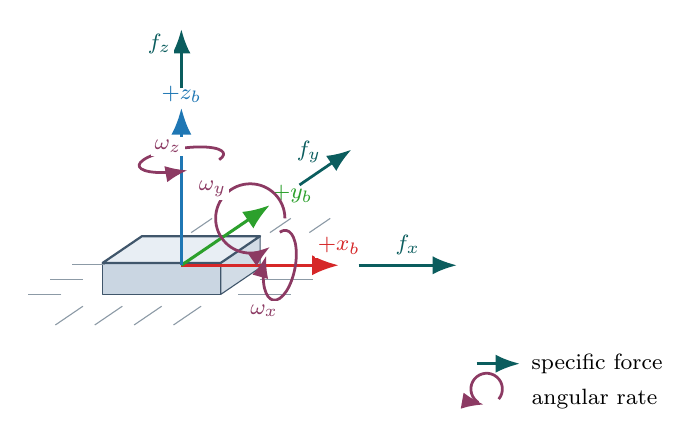
\begin{tikzpicture}[
  % This maps TikZ's logical 3D coordinates into the 2D page.
  % x points horizontally right, y points diagonally up-right, and z points up.
  % Changing these three basis vectors changes the viewing angle.
  x={(1.00cm,0.00cm)},
  y={(0.50cm,0.34cm)},
  z={(0.00cm,1.00cm)},
  % Rounded joins make the small package and arrows look less harsh.
  % line cap=round,
  line join=round,
]

% Origin of the body frame. All axis arrows start here.
\coordinate (O) at (0,0,0);

% Corners of the rectangular IMU package.
% A-D are the lower corners and E-H are the matching upper corners.
\coordinate (A) at (-0.75, -0.50, -0.20);
\coordinate (B) at ( 0.75, -0.50, -0.20);
\coordinate (C) at ( 0.75,  0.50, -0.20);
\coordinate (D) at (-0.75,  0.50, -0.20);
\coordinate (E) at (-0.75, -0.50,  0.20);
\coordinate (F) at ( 0.75, -0.50,  0.20);
\coordinate (G) at ( 0.75,  0.50,  0.20);
\coordinate (H) at (-0.75,  0.50,  0.20);

% Draw the visible faces of the IMU package. The order matters: side faces first,
% then the top face, so the top outline stays crisp.
\filldraw[fill=chipside, draw=chipline] (A) -- (B) -- (F) -- (E) -- cycle;
\filldraw[fill=chipside!85!white, draw=chipline] (B) -- (C) -- (G) -- (F) -- cycle;
\filldraw[fill=chipfill, draw=chipline, line width=0.8pt] (E) -- (F) -- (G) -- (H) -- cycle;

% Decorative pins on the near and far long edges.
\foreach \p in {-0.75,-0.25,0.25,0.75} {
  \draw[chipline!60] (\p,-1.00,-0.18) -- (\p,-1.70,-0.18);
  \draw[chipline!60] (\p, 1.75,-0.18) -- (\p, 2.28,-0.18);
}

% Decorative pins on the short edges.
\foreach \p in {-0.55,0,0.55} {
  \draw[chipline!60] (-1.25,\p,-0.18) -- (-1.67,\p,-0.18);
  \draw[chipline!60] ( 1.00,\p,-0.18) -- ( 1.67,\p,-0.18);
}

% Package label.
% \node[partlabel] at (0,-0.50,-0.33) {IMU};

% Body-frame axes. These are the positive x/y/z directions of the IMU's local
% frame, not necessarily north/east/down or any global navigation frame.
\draw[axis, bodyred] (O) -- (2,0,0) node[channel, above=2pt] {$+x_b$};
\draw[axis, bodygreen] (O) -- (0,2.25,0) node[channel, above right=-1pt] {$+y_b$};
\draw[axis, bodyblue] (O) -- (0,0,2) node[channel, above] {$+z_b$};

% Accelerometer channels. An ideal strapdown IMU reports specific force along
% each body axis, so these arrows are parallel to +x_b, +y_b, and +z_b.
% They are offset from the axes only to keep the labels and arrows visible.
\draw[force] (2.25, 0, 0.0) -- (3.5,0,0)
  node[channel, midway, above=2pt] {$f_x$};
%\draw[force] (-0.50,0.12,0.62) -- (-0.50,1.32,0.62)
\draw[force] (0,3.0,0) -- (0.0,4.32,0.0)
  node[channel, midway, above left=0pt] {$f_y$};
\draw[force] (0.0,0.0, 2.25) -- (0.0,0.0, 3.0)
  node[channel, near end, left=2.pt] {$f_z$};

% Gyro channels. Each loop is drawn in the plane perpendicular to the axis it
% measures, following the right-hand-rule positive rotation sense.

% Positive roll-rate channel about +x_b. The temporary scope makes a 2D drawing
% plane normal to x, located at x = 1.25.
\begin{scope}[canvas is yz plane at x=1.25]
  \draw[rate] (0.00,0.42) arc[start angle=90, end angle=-215, radius=0.42];
  \node[channel, text=ratecolor] at (-0.40,-0.44) {$\omega_x$};
\end{scope}

% Positive pitch-rate channel about +y_b.
\begin{scope}[canvas is xz plane at y=1.75]
  \draw[rate] (0.44,0.00) arc[start angle=0, end angle=305, radius=0.44];
  \node[channel, text=ratecolor] at (-0.48,0.38) {$\omega_y$};
\end{scope}

% Positive yaw-rate channel about +z_b.
\begin{scope}[canvas is xy plane at z=1.34]
  \draw[rate] (0.48,0.00) arc[start angle=0, end angle=305, radius=0.48];
  \node[channel, text=ratecolor] at (-0.42,0.50) {$\omega_z$};
\end{scope}

% Compact legend. This scope deliberately switches back to plain 2D page
% coordinates so the legend is not skewed by the 3D viewing transform.
\begin{scope}[x={(1cm,0cm)}, y={(0cm,1cm)}, shift={(3.75,-1.25)}]
  \draw[force] (0,0) -- (0.55,0);
  \node[channel, anchor=west] at (0.65,0) {specific force};
  \draw[rate] (0.28,-0.45) arc[start angle=-40, end angle=260, radius=0.2];
  \node[channel, anchor=west] at (0.65,-0.45) {angular rate};
\end{scope}

\end{tikzpicture}
\end{document}
